\documentclass[]{article}
\usepackage[main=english,french]{babel}
\usepackage[utf8x]{inputenc}
\usepackage{enumitem}  
\usepackage{listings}
\usepackage{arydshln}
\usepackage{amsmath}
\usepackage{cases}  
\usepackage{cite}
\usepackage{graphicx}
\usepackage{dsfont}
\usepackage{float}
\usepackage[bottom]{footmisc}
 \graphicspath{{images/}}
%opening
\title{Stationary and non-stationary sinusoidal model synthesis with phase vocoder and FFT$^{-1}$}
\author{Cl\'ement Cazorla, Vincent Chrun, Bastien Fundaro, Cl\'ement Maliet \\ENSEEIHT - 3EN TSI 2016-2017}


\begin{document}

\maketitle

\begin{abstract}
The present document is to serve as both a technical report and a documentation for the code produced during the long project. As such the first part will explain the theoretical framework and the state-of-the-art of the field. The second part will give some insight about the code structure and the conventions that were adopted and last but not least, the third part will serve as an actual documentation and details every class, methods and attributes.
\end{abstract}
 \vspace{5cm}
	\begin{figure}[H]
		\centering
		\includegraphics[scale=0.28]{ag.png}
	\end{figure}
	\begin{figure}[H]
		\centering
		\includegraphics[scale=0.28]{enseeiht.png}
	\end{figure}

\newpage
\tableofcontents


\newpage
\part{Introduction}\label{sec:introduction}

\section{The company}\label{sec:the-company}
For this project we work with Audiogaming. Audiogaming is a start-up company which creates audio
plug-in for movies and video games. They are base in Toulouse and Paris.
\begin{figure}[H]
	\centering
	\includegraphics[scale=0.19]{AudioFire_screen.png}
	\caption{\it Audiofire: audio plug-in that recreates fire sound}
\end{figure}

\section{Objective}\label{sec:objective}

The objective of the project is to use
inverse Fourier transform to synthesize a sound. There are two
parts in this process: the Analysis and the Synthesis.
	\begin{figure}[H]
		\centering
		\includegraphics[scale=0.4]{Analysis_Synthesis.png}
		\caption{\it General approach for modifying a sound in the spectral domain}
	\end{figure}

Our objectives were to focus on the synthesis. We supposed that the analysis part is done and that we know all the parameters. The work is divided into two parts : the stationary synthesis and the non-stationary synthesis. 
\section{Context of the project}\label{sec:context-of-the-project}
We had 6 weeks to do this work. As a beginning, we had the work of the previous group which worked on this project in 2015. They had done an analysis estimator of sinus parameters and sinus generation with those
parameters (only stationary) in Python and some research on the Non-stationary synthesis with the LUT of lobes in Matlab.
We imposed to ourself an Object Oriented Programming tree structure in Python, in that way the code will be easier to use by the client and the next group which will work on this project. This structure will be described in details in this report. 
\section{Work environment and project management}\label{sec:work-environment-and-project-management}
\subsection{Work environment}
We used PyCharm to program in Python, Slack to communicate with our supervisor (ask questions, send some quick results, plan a meeting...). An other important tool was GitHub, we used it to share our codes and to work all at the same time in the same project. 
	\begin{figure}[H]
		\centering
		\includegraphics[scale=0.4]{all_softwares.png}
		\caption{ {\it PyCharm} as Python IDE , {\it Slack} to communicate,{\it GitHub} to stock the codes and have a versionning, {\it Freedcamp} to plan the project events }
	\end{figure}

\subsection{Project management (Gantt chart)}
\begin{figure}[H]
	\centering
	\rotatebox{90}{\includegraphics[scale=0.44]{Gantt.png}}
\end{figure}

\newpage
\part{Sound synthesis in the frequency domain}
\section{General analysis/synthesis approach}\label{part:general-approach}
\subsection{Additive Synthesis (Time Domain)}\label{sec:additive-synthesis-(time-domain)}
In signal processing, about as much work has been done in analysing sounds as in synthesizing them. The most common approach is to assimilate the sound to a finite sum of time varying sinusoids, which are called partials \cite{quatieri2002audio} added to a residual, that is, a stochastic process equivalent to a noise:
\begin{equation}
s(t) = \sum_{i=1}^{K}\alpha_i(t) \sin(2\pi f_i(t) t + \phi_{i}) + e(t)
\end{equation}
Where the amplitude $\alpha_i(t)$ and the frequency $f_i(t)$ are smooth slowly varying functions.\\
Although in most cases, that is speech or musical instruments synthesis, the residual contribution is not negligible compared to the partials \cite{quatieri2002audio, rodet1992spectral} one can, in a first time, set the residual term to zero\footnote{In fact, the sinusoidal plus residual model is a direct consequence of the source/filter model \cite{mcaulay1986speech}, the synthesis of the residual term is thus more or less equivalent to filtering a white noise, which is, in its naive resolution, simpler than the sinusoids synthesis. This is why we mainly focus on the sinusoidal synthesis despite the non negligible nature of the residual term.}.\\
This synthesis method is also motivated by the fact that a great amount of research has been done towards analysing such sound models \cite{rodet1992spectral, depalle1993tracking}. The most common and obvious approach consists in adding a number of independent oscillator to reproduce the sound, each one of them being controlled independently.\\
\\
However the main issue at stake is that it is very costly to implement, so it is impossible to use in real-time applications. A solution would be to generate the sines in frequency domain, using the parameters given by the analysis.\\

\begin{figure}[H]
	\centering
	{\includegraphics[scale=0.4]{additif.png}}
	\caption{\it The additive synthesis}
\end{figure} 
\medskip

\subsection{General framework}\label{sec:general-framework}

The first step of the method is the analysis. The aim is to extract the parameters of the signal (magnitude, phase, frequency).
First of all, we window the signal in order to maximize the energy in the main lobe, with Hanning, Blackman-Harris... window for instance (Figure \ref{windowing}):

\begin{figure}[H]
	\centering
	{\includegraphics[scale=0.4]{slide1.png}}
	\caption{\it Windowing step}
	\label{windowing}
\end{figure}

\medskip

Then, we apply a STFT (Short Time Fourier Transform) to extract the coefficients.  We assume each peak represents a sinusoid, and we use a particular case of STFT called STPT, that detects peaks in the signal and that applies the STFT in the areas that are close to the peaks and sets the rest of the signal to zero. It is a simplest version of STFT, because we neglect the residual part of the signal by only considering the periodic part of the signal. This is less costly and works quite well, except in case of transitional signal because it is very difficult to model with a finite sum of sines. 

\begin{figure} [H]
	\centering
	{\includegraphics[scale=0.7]{slide2.png}}
	\caption{\it Peaks detection}
\end{figure}
\medskip
Finally, we synthesize the new signal by FFT$^{-1}$ and we compare it to the original signal we applied the analysis to.

\begin{figure}[H]
	\centering
	{\includegraphics[scale=0.7]{synthesisstep.png}}
	\caption{\it Synthesized frame vs Original frame}
\end{figure}

The image below is a little sum up of the method:

\begin{figure}[H]
	\begin{center}
	{\includegraphics[scale = 0.8]{schema.png}}
	\caption{\it Block diagram of a higher-level spectral-processing framework}
	\end{center}
\end{figure}

\newpage

\subsection{Phase Coherence}\label{phase-coherence}
The phase becomes a problem when we are synthesizing a signal, even a simple sinusoid, because for each frame we create a "different" sinusoid with the same parameters. That is not what we want, we want to create a single sinusoid : 
\begin{figure} [H]
	\centering
	\includegraphics[scale = 0.2]{coherentphase.png}
	\caption {\it Coherent phase (above) vs. Incoherent phase (below) between frames}
\end{figure}
When we listen to a signal which phase is incoherent between frames (vertical jump) it will sound as "pops".  This is something very unpleasant to listen to. We need to do something to make sure there is no discontinuity. Thus, correcting the phase is absolutely necessary. \\
In the stationary case, it is something easy to do. Knowing the exact frequency and for each frame, we advance the phase of $2\pi \tilde{f} R_a$  \footnote{To see details of the theoretical phase advance for the stationary case, please refer to the appendix \ref{theoretical_phase_advance} page \pageref{theoretical_phase_advance}.}.
\section{Sinusoid synthesis in the frequency domain}

\subsection{Stationary Case}
Most stationary signals can be decomposed in a sum of partials with seldom loss in perception :
\begin{equation}
s(n) = \sum_{i=1}^{K}\alpha_i \sin(2\pi \tilde{f_i} n + \phi_{i})
\end{equation}
If all three parameters $\alpha_i$, $\tilde{f_i}$ and $\phi_{i}$ are known for each partial, perfect reconstruction is thus possible.\\
It is first needed to compute the Fourier transform of a given frame. Let $w_{t_a}(n)$ be an analysis window starting at $t_a = kR_a$ where $R_a$ is called the \emph{hop size}. The resulting spectral frame is:
\begin{equation}
S_{t_a}(m) = \text{DFT}[s](m) \ast W_{t_a}(m)
\end{equation}
Where $W_{t_a}(m)$ is the DFT of the window $w_{t_a}$. Under the right assumptions on the window phase\footnote{Which involves circular shift to cancel the phase shift \cite{arfib2002time}.}, the spectrum consists in main and secondary lobes (which originates directly from $W_{t_a}(m)$) convolved at the sinus amplitude, phase and frequency.\\
However since most of the energy is concentrated in the main lobe\footnote{At the condition that $w_{t_a}$ is not rectangular.}, one can omit the side lobes with little to no error, ever more so since most of the error is made on the edges of the temporal frame where the amplitude is small. In the stationary case, every main lobes are identical in shape, this means that one can synthesise a spectrum by copying a precomputed lobes onto the relevant bins of the FFT. This makes the process computationally light since only 9 points of the main lobes are sufficient \cite{rodet1992spectral}, although our method used 11 for further precision.\\
\begin{figure}
	\centering
	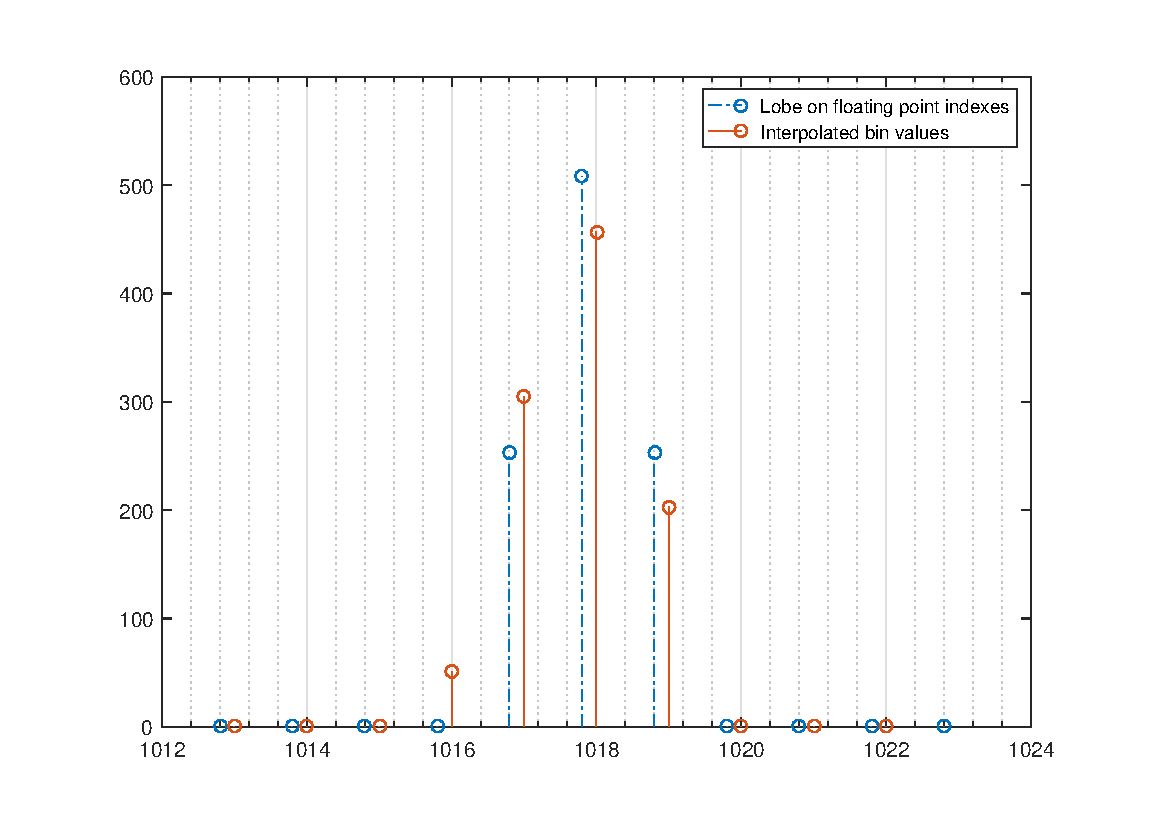
\includegraphics[scale=0.4]{Interpolation.eps}
	\caption{\it Interpolation of stored lobe values onto the FFT bins.}
	\label{interpBin}
\end{figure}
Interpolation is necessary to fill the bins because the sinusoid frequency bin $\hat{f_i}$ is unlikely to fall on an integer bin number ($\hat{f_i} = \tilde{f_i}\times N$ with $N$ the FFT size) as illustrated in figure \ref{interpBin}, this step allows for a good precision in frequency without the need for zero-padding the spectrum, thus increasing performance.\\
The phase is set at a common value for every bins of the lobe, on the rational that they all represents the contribution of the same sinusoid. Note that the phase used is the original phase $\phi_{i}$ corrected from the windowing effects and advanced by the time passed, to ensure phase coherence as explained in section \ref{phase-coherence}, that is to say that:
\begin{equation}\label{statPhaseShift}
\phi_{lobe} = \hat{\phi_{i}} + k\times 2\pi \tilde{f_i} R_a
\end{equation}
Where $\hat{\phi_{i}}$ denote the window-corrected phase, $2\pi \tilde{f_i} R_a$ the phase advance for a single hop at frequency $\tilde{f_i}$ and $k$ s.t $t_a = k\times R_a$.
\subsection{Quasi-Stationary Case}\label{quasi-stationary-case}
Although most of what has been said before still holds in the quasi-stationary case, a few changes have to be made so that the synthesis work.\\
The signal is a non stationary signal which can be approximately considered as stationary given a small enough window:
\begin{equation}
s(n)\cdot \mathds{1}_{[t_a^{u-1}, t_a^u]} \simeq \sum_{i=1}^{K}\alpha_i^{u} \sin(2\pi \tilde{f_i^{u}} n + \phi_{i}^u)
\end{equation}
However, while the synthesised spectrum amplitude remain unchanged, the phase has to be corrected to take into account both the fact that the sinusoid initial phase $\phi_i$ has to be passed along the sinusoid track if its frequency where to change, and phase advance corrections due to the non-stationary nature of the signal. \\
Indeed, although we assume the signal to be stationary in a short frame, this mainly implies that the synthesised lobe corresponding to the sinusoid is identical to a stationary sinusoid lobe. However, because of the recursive nature of the synthesis phase, errors in phase advances due to either a loss of precision in frequency estimation\footnote{As one will see in the true non-stationary case, amplitude and phase shifts have significant influence one the lobe appearance} or applying stationary phase shift as seen in (\ref{statPhaseShift}), may lead to significant phase deviation after a few iteration. This may in turn leads to significant phase de-coherence in the case of a note onset, that is the appearing of a new sinusoid.\\
One proposed method relies on a Phase Vocoder\footnote{See annex \ref{phase-vocoder-annex} page \pageref{phase-vocoder-annex} for more informations on Phase Vocoders.} to take into account and corrects unexpected phase shift due to non-stationarity in the pre-analysed reference signal. The phase is then set to the reference signal phase corrected for a possible difference in analysis and synthesis hop size. However, because we rely on the analysis phase to ensure correct phase propagation, the method loses the initial flexibility of a true sinusoidal model.\\
Another possible approach is to pass the true theoretical phase advances along the track. Although it implies that one is able to track the sinusoid evolution (the complexity of which is substantial \cite{mcaulay1986speech, serra1989system, karrer2006phavorit}), this has the advantage of keeping a truly sinusoidal framework as in the stationary case.\\
The following has not been implemented, but the idea is to estimate coarsely the non-stationary \emph{Frequency Change Rate} ($\psi$) between two frame and apply non-stationary sinusoid phase shift.\\
The linear chirp is written as follow\footnote{The non-stationary case hypotheses and framework can be found in the section \ref{non-stationary-case} below.}:
\begin{equation}
s(t) \propto \sin\left(2\pi\left(f  + \frac{1}{2\pi}\frac{\psi}{2} t\right)t + \phi_a\right)
\end{equation}
Thus the frequency shift between two consecutive frames is:
\begin{equation}
\begin{split}
\Delta f & = f_{H_a} - f_0\\
& = f_0 + \frac{\psi}{4\pi}H_a - f_0\\
& = \frac{\psi}{4\pi}H_a
\end{split}
\end{equation}
We can thus estimate $\psi$ between two frames:
\begin{equation}
\hat{\psi}_{t_a} = \frac{4\pi}{H_a}\left(f_{(t_a + H_a)} - f_{t_a} \right)
\end{equation}
The estimated phase advance (\ref{phaseadvanceNonStat}) computed in annex \ref{theoretical_phase_advance_nonstat} page \pageref{theoretical_phase_advance_nonstat} is thus:
\begin{equation}
\Delta \Phi_{f}^{t_a} = 2\pi f_{t_a} H_a + \frac{\psi}{2}H_a^2 = 2\pi H_a\left(f_{t_a} + f_{(t_a + H_a)} - f_{t_a} \right) = 2\pi f_{(t_a + H_a)} H_a
\end{equation}
\subsection{Non-Stationary Case}\label{non-stationary-case}

\subsubsection{The look-up table}\label{The look-up table}
\hspace{15pt}
The principle of the method is to create a regular or irregular ACR/FCR (Amplitude Change Rate/Frequency Change Rate) grid. For each point of the grid which is represented by an ACR/FCR couple, we store an eleven-point main lobe in the look-up table. Hence, the size of the look-up table is equal to number\_of\_ACR times number\_of\_FCR. Then, we can find the lobe for the couple of ACR/FCR we want by interpolating.
\begin{figure}[H]
	\centering
	\includegraphics[scale=0.6]{grid.png}
	\caption{\it Interpolation of stored lobe values onto the FFT bins.}
\end{figure}

The look-up table should not be too big so it does not take too much memory. As a consequence, we have to find a compromise between the size of the look-up table and the precision of the interpolation.

\begin{figure}[H]
	\centering
	\includegraphics[scale=0.8]{LUT.png}
	\caption{\it Interpolation of stored lobe values onto the FFT bins.}
\end{figure}

We tested different kind of interpolation because the interpolation that gives the best results is not the same for the magnitude as for the phase. Finally, we figured out that the interpolation that works better for the magnitude in the cubic one, whereas the one that works better for the phase is the linear one which sounds quite logical giving the form of the curves. The user can choose the interpolation method he wishes for both amplitude and phase.



\newpage
\part{Results}
\section{Stationary Case}\label{sec:stationary-results}
\section{Non-Stationary Case}\label{non-stationary-results}

\newpage
\part{Code structure and conventions}\label{sec:code-structure-and-conventions}

\section{Conventions}\label{sec:conventions}

In this section we remind the reader of a few coding convention necessary to ensure a seamless work flow and a bug free program as much as possible.
Files should contains an entire module (as described in \ref{sec:general-structure}) not just a single class to limit the number of files and ease the bug tracking.
Imports in files should be kept to a minimum and left in namespaces (do not use the \lstinline[columns=fixed,language=Python]|from module import *| syntax). It is preferable to import a whole module if more than three elements from the module are needed in the file, otherwise consider the \lstinline[columns=fixed,language=Python]|from module import element1, element2| syntax to avoid unnecessary memory flooding. If conflicts exists, notwithstanding the number of elements needed, the whole modules are to be loaded with a namespace.
Namespaces may be abbreviated to the programmer's convenience however some abbreviation are to be universally respected :
\begin{enumerate}[label=(\roman*)]
	\item \texttt{numpy} should always be imported as \texttt{np}
	\item \texttt{matplotlib.pyplot} should always be imported as \texttt{plt}
\end{enumerate}

Finally math functions should always come from the numpy module and not python's math module to guarantee a universal behaviour across the program.

\subsection{Naming conventions}\label{sec:naming-conventions}

Naming conventions are freely adapted from Python recommended conventions defined in PEP8 \cite{pep8}, as such :
\begin{enumerate}[label=(\roman*)]
	\item \emph{Class} should be named in \texttt{CapitalizedWord}
	\item \emph{Methods} and \emph{functions} should be named in \texttt{lower\_case\_with\_underscores}
	\item \emph{Attributes} and \emph{variables} should be names in \texttt{lower\_case\_with\_underscores}
	\item \emph{Instantiation} following the fact that everything is an object in python should be named as \emph{variables}.
\end{enumerate}
Moreover during class declaration, the following principles should be adopted :
\begin{enumerate}[label=(\roman*)]
	\item Non-public methods and attributes should use one leading underscore.
	\item Elements that conflicts with python reserved name should use one trailing underscore rather that simplification or a misspelling.
	\item Accessors or mutators using one leading underscore should be interpreted as properties of their associated attribute. As such it should be guaranteed that they induce a low computational cost.
	\item Non-public elements that should not be inherited or may cause conflicts during inheritance should use two leading underscore and make use of Python name-mangling.
\end{enumerate}
To seamlessly manipulate both \emph{stationary} and \emph{non stationary} models, class that are inherited in two versions are preceded with either \texttt{Stationary} are \texttt{NonStationary} respectively.
\subsection{Spectrum and sinusoids parameters classes}\label{sec:spectrums-and-sinusoids-parameters}
Because many spectra, main lobes and sinusoidal model parameters have to be traded between modules we created two classes, respectively \texttt{Spectrum} and \texttt{Parameters}. They mainly serve as containers, holding the data and returning them in a point wise fashion.
This way we can prevent conflicts and errors that would come from a non-uniform data sharing protocol and as well ensure that every operation performed on either spectra or parameters are made following the same principles and algorithms.
\subsubsection{Spectrum}
\texttt{%
\begin{tabular}{|lc|}
	\hline
	Spectrum & \\
	\hline
	\hline
	\_amplitude : np.array & \\
	\_phase : np.array  & \\
	\_nfft : int  & \\
	\hdashline
	\_\_init\_\_(self, amplitude, phase) & \\
	\_\_add\_\_(self, other) & \\
	\_\_iadd\_\_(self, other) & \\
	\_\_mul\_\_(self, other) & \\
	\_\_imul\_\_(self, other) & \\
	from\_complex\_spectrum(cls, complex\_spectrum) & @classmethod\\
	void\_spectrum(cls) & @classmethod\\
	set\_spectrum(self, amplitude, phase, & \\ \hspace{10mm} start\_bin=None, stop\_bin=None) & \\
	set\_complex\_spectrum(self, complex\_spectrum, & \\ \hspace{10mm} start\_bin=None, stop\_bin=None) & \\
	get\_amplitude(self, k) & \\
	get\_phase(self, k) & \\
	get\_nfft(self) & \\
	\hline
\end{tabular}} \medskip\newline
The Spectrum class stores a spectrum in amplitude and phase, however it may be created or changed from a complex \texttt{np.array} respectively with the class method \texttt{from\_complex\_spectrum} and the method \texttt{set\_complex\_spectrum}. Those two methods may take optional parameters start\_bin and stop\_bin if one need to update only a part of the spectrum, for example a single lobe. The class checks that the given data are consistent upon instantiation.
The $+$ operation as well as the $+=$ operation have been defined between two \texttt{Spectrum} objects and between a \texttt{Spectrum} object and an array of complex numbers.\\
The $\times$ operation as well as the $\times=$ operation have been defined between a \texttt{Spectrum} object and an array of complex numbers.
Addition and multiplication attempts between other data type will result in a \texttt{NotImplementedError} exception.
\subsubsection{Parameters}
\texttt{%
	\begin{tabular}{|lc|}
		\hline
		Parameters & \\
		\hline
		\hline
		\_amplitudes : np.array & \\
		\_frequencies : np.array & \\
		\_phases : np.array  & \\
		\_number\_sinuses : int  & \\
		\hdashline
		\_\_init\_\_(self, amplitudes, frequencies, phases) & \\
		get\_amplitude(self, k) & \\
		get\_frequency(self, k) & \\
		get\_phase(self, k) & \\
		get\_number\_sinuses(self) & \\
		\hline
\end{tabular}} \medskip\newline
The Parameters class is more of a structure than a class and only contains the stationary sinusoidal model parameters and their respective accessors. It also stores the number of sinuses and checks that the given data are consistent upon instantiation.\\
In the stationary sinusoidal model the signal $s(t)$ is defined as follow\footnotemark[1] :
\begin{equation*}
	s(n) = \sum_{i=1}^{N_{sinus}} \alpha_i \sin(2\pi \tilde{f_i} n+ \phi_i)
\end{equation*}
with $\tilde{f_i} = \frac{f_i}{f_s}$ the normalised frequency.\\
We then store the parameters as follows :
\begin{description}
	\item[\_amplitudes] stores the $\alpha_i$
	\item[\_frequencies] stores the $\tilde{f_i}$
	\item[\_phases] stores the $\phi_i$
\end{description}
\subsubsection{NonStationaryParameters}
\texttt{%
	\begin{tabular}{|lc|}
		\hline
		NonStationaryParameters(Parameters) & \\
		\hline
		\hline
		\_acrs : np.array & \\
		\_fcrs : np.array & \\
		\hdashline
		\_\_init\_\_(self, amplitudes, frequencies, phases, acrs, fcrs) & \\
		get\_acr(self, k) & \\
		get\_fcr(self, k) & \\
		\hline
\end{tabular}} \medskip\newline
The stationary sinusoidal model can be extended to the first order development to better model fast amplitude and frequency change over time. The signal $s(t)$ can then be expressed as a sum of linearly varying chirps\footnotemark[1] :
\begin{equation*}
	s(n) = \sum_{i=1}^{N_sinus} (\alpha_i + \mu_i \cdot nT_s) \sin(2\pi \tilde{f_i} n + \frac{\psi_i}{2} (nT_s)^2 + \phi_i)
\end{equation*}
Where we define the \textbf{Amplitude Change Rate} $\mu$ and the \textbf{Frequency Change Rate} $\psi$. \\
Thus we inherit the \texttt{Parameters} class to add the two additional parameters as follow :
\begin{description}
	\item[\_acrs] stores the $\mu_i$
	\item[\_fcrs] stores the $\psi_i$
\end{description}
\footnotetext[1]{Please look up section \ref{non-stationary-case} page \pageref{non-stationary-case} for more details}
\section{Code structure}\label{sec:code-structure}
\subsection{General structure}\label{sec:general-structure}
\subsection{Class structure}\label{sec:class-structure}


\newpage
\part{Documentation}\label{sec:documentation}
\section{Core module}
\subsection{Synthesizer}

\texttt{%
	\begin{tabular}{|lc|}
		\hline
		Synthesizer & \\
		\hline
		\hline
		\_window\_size : float & \\
		\_window\_type : float & \\
		\_nfft : float  & \\
		\_analysis\_hop : float & \\
		\_synthesis\_hop : float & \\
		\_current\_parameters : Parameters & \\
		\_past\_parameters : Parameters & \\
		\_fs : float & \\
		\_past\_spectrum : Spectrum & \\
		\_current\_spectrum : Spectrum & \\
		\hdashline
		\_\_init\_\_(self, window\_size, window\_type, zero\_padding\_factor, analysis\_hop, 
		\\ synthesis\_hop, current\_parameters, fs=None) & \\
		\_\_del\_\_(cls) & \\
		reset\_synthetizer (self, window\_size, window\_type, zero\_padding\_factor, \\
		analysis\_hop, synthesis\_hop, current\_parameters, fs) & \\
		get\_next\_frame(self) & \\
		set\_next\_frame(self, next\_parameters) & \\
		\_set\_window\_size(self, window\_size) & \\
		\_set\_window\_type(self, window\_type) & \\
		\_set\_analysis\_hop(self, analysis\_hop) & \\
		\_set\_synthesis\_hop(self, synthesis\_hop) & \\
		\_set\_current\_parameters(self, current\_parameters) & \\
		\_get\_current\_spectrum(self) & \\
		\_set\_current\_spectrum(self, new\_spectrum) & \\
		\hline
\end{tabular}} \medskip\newline

The aim of the Synthesizer is to set all the parameters which are used to make the synthesis, that is to say the type and the size of the window, the FFT number and the hop size for the analysis and the synthesis. Moreover, it returns the spectrum of the signal.

\subsection{StationarySynthesizer}

\texttt{%
	\begin{tabular}{|lc|}
		\hline
		StationarySynthesizer & \\
		\hline
		\hline
		\_window\_size : float & \\
		\_window\_type : float & \\
		\_nfft : float  & \\
		\_analysis\_hop : float & \\
		\_synthesis\_hop : float & \\
		\_current\_parameters : Parameters & \\
		\_past\_parameters : Parameters & \\
		\_fs : float & \\
		\_past\_spectrum : Spectrum & \\
		\_current\_spectrum : Spectrum & \\
		\_spectrum\_generator : StationarySpectrumGenerator & \\
		\hdashline
		\_\_init\_\_(self, window\_size, window\_type, zero\_padding\_factor, analysis\_hop, \\
		 synthesis\_hop, current\_parameters, fs=None) & \\
		get\_next\_frame(self) & \\
		inverse\_fft(self, current\_spectrum) & \\
		\hline
\end{tabular}} \medskip\newline


\subsection{NonStationarySynthesizer}

\texttt{%
	\begin{tabular}{|lc|}
		\hline
		NonStationarySynthesizer & \\
		\hline
		\hline
		\_window\_size : float & \\
		\_window\_type : float & \\
		\_nfft : float  & \\
		\_analysis\_hop : float & \\
		\_synthesis\_hop : float & \\
		\_current\_parameters : NonStationaryParameters & \\
		\_past\_parameters : NonStationaryParameters & \\
		\_fs : float & \\
		\_past\_spectrum : Spectrum & \\
		\_current\_spectrum : Spectrum & \\
		\_spectrum\_generator : StationarySpectrumGenerator & \\
		\hdashline
		\_\_init\_\_(self, window\_size, window\_type, zero\_padding\_factor, analysis\_hop, \\
		 synthesis\_hop, current\_parameters, fs=None) & \\
		get\_next\_frame(self) & \\
		inverse\_fft(self, current\_spectrum) & \\
		\hline
\end{tabular}} \medskip\newline


\section{Spectrum generation module}\label{sec:spectrum-generation-module}
\subsection{SpectrumGenerator}\label{sec:spectrumgenerator}

\texttt{%
	\begin{tabular}{|lc|}
		\hline
		SpectrumGenerator & \\
		\hline
		\hline
		\_parameters : Parameters & \\
		\_nfft : np.float & \\
		\_spectrum : Spectrum & \\
		\_window\_size : np.float & \\
		\_analysis\_hop : np.float & \\
		\hdashline
		\_\_init\_\_(self, window\_size, parameters, nfft, analysis\_hop)&\\
		\_add\_lobe(self, k, lobe) & \\
		\_set\_window\_size(self, window\_size) & \\
		\_set\_window\_type(self, window\_type) & \\
		\_get\_parameters(self, new\_parameters) & \\
		\_get\_spectrum(self) & \\
		\hline
\end{tabular}} \medskip\newline


 
The aim of this class is to generate a synthetic spectrum from known parameters (amplitudes, phases, frequencies). This class is divided into two subclasses that generate stationary and non-stationary spectrums.\\

\subsection{StationarySpectrumGenerator}\label{sec:stationaryspectrumgenerator}

\texttt{%
	\begin{tabular}{|lc|}
		\hline
		StationarySpectrumGenerator (SpectrumGenerator) & \\
		\hline
		\hline
		\_parameters : Parameters & \\
		\_nfft : np.float & \\
		\_spectrum : Spectrum & \\
		\_window\_size : np.float & \\
		\_analysis\_hop : np.float & \\
		\_lobe\_generator : StationaryLobeGenerator & \\
		\hdashline
		\_\_init\_\_(self, window\_size, parameters, nfft, analysis\_hop)&\\
		\_add\_lobe(self, k, lobe) & \\
		\hline
\end{tabular}} \medskip\newline


\subsection{NonStationarySpectrumGenerator}\label{sec:nonstationaryspectrumgenerator}
\texttt{%
	\begin{tabular}{|lc|}
		\hline
		NonStationarySpectrumGenerator (SpectrumGenerator) & \\
		\hline
		\hline
		\_parameters : Parameters & \\
		\_nfft : np.float & \\
		\_spectrum : Spectrum & \\
		\_window\_size : np.float & \\
		\_analysis\_hop : np.float & \\
		\_lobe\_generator : NonSationaryLobeGenerator & \\
		\_regular\_lut : np.array & \\
		\hdashline
		\_\_init\_\_(self, window\_size, parameters, nfft, analysis\_hop)&\\
		\_add\_lobe(self, k) & \\
		\hline
\end{tabular}} \medskip\newline

This class has not been made yet, but the goal is the same as for the StationarySpectrumGenerator.
\subsection{LobeGenerator}\label{sec:lobegenerator}

\texttt{%
	\begin{tabular}{|lc|}
		\hline
		LobeGenerator & \\
		\hline
		\hline
		\_window\_type : np.float & \\
		\_window\_size : np.float & \\
		\_nfft : np.float & \\
		\_window : np.array &\\
		\_lobe : Spectrum & \\
		\hdashline
		\_\_init\_\_(self, window\_type, window\_size, nfft) &\\
		\_set\_window\_size(self, window\_size) & \\
		\_set\_window\_type(self, window\_type) & \\
		\_gen\_lobe(self) & \\
		\_get\_lobe & \\
		\hline
\end{tabular}} \medskip\newline
This class generates a 11 points main lobe.

\subsubsection{StationnaryLobeGenerator}\label{sec:stationnarylobegenerator}

\texttt{%
	\begin{tabular}{|lc|}
		\hline
		StationaryLobeGenerator(LobeGenerator) & \\
		\hline
		\hline
		\_window\_type : np.float & \\
		\_window\_size : np.float & \\
		\_nfft : np.float & \\
		\_window : np.array &\\
		\_lobe : Spectrum & \\
		\_gen\_lobe : Spectrum & \\
		\hdashline
		\_\_init\_\_(self, window\_type, window\_size, nfft) &\\
		\_gen\_lobe(self) & \\
		\hline
\end{tabular}} \medskip\newline

\subsubsection{NonStationaryLobeGenerator}\label{sec:nonstationarylobegenerator}
\texttt{%
	\begin{tabular}{|lc|}
		\hline
		NonStationaryLobeGenerator(LobeGenerator) & \\
		\hline
		\hline
		\_abscisse : np.array & \\
		\_ordonnee : np.array & \\
		\_interpolated\_lobe : np.array & \\
		\_regular\_grid : np.array & \\
		\_domain : np.array & \\
		\_number\_acr : np.float & \\
		\_number\_fcr : np.float & \\
		\_number\_points : np.float & \\
		\_LUT : np.array & \\
		\_gen\_lobe : Spectrum & \\
		\hdashline
		\_\_init\_\_(self, regular\_grid, acr\_domain, fcr\_domain, number\_acr, number\_fcr, window\_type,\\ window\_size, nfft, fs=None, method\_a=None, method\_p=None, method\_f=None) &\\
		\_gen\_uniform\_lut(self) & \\
		\_gen\_non\_uniform\_lut(self) & \\
		\_gen\_lobes\_legacy(self, i, j, acr, fcr, t, n) & \\
		\_gen\_lobe(self) & \\
		\_get\_lobe(self) & \\
		\_interpolate\_lobe(self, acr, fcr, method\_a=None, method\_p=None, method\_f = None)) & \\
		\hline
\end{tabular}} \medskip\newline
\\

The aim is to generate a LUT with a uniform or a non-uniform grid, and to generate a lobe for a given ACR/FCR couple by interpolating with existing lobes of the LUT. The user must chose the kind of interpolation he or she wants to use for magnitude, phase and frequency. Besides, he can choose the size of the LUT to build by giving the number of ACRs and FCRs.
\section{Phase Vocoder module}\label{sec:phase-vocoder-module}
\subsection{PhaseVocoder}\label{sec:phasevocoder}
\texttt{%
	\begin{tabular}{|lc|}
		\hline
		PhaseVocoder & \\
		\hline
		\hline
		\_analysis\_hop : int & \\
		\_synthesis\_hop : int & \\
		\_omega : np.array  & \\
		\_past\_analysis\_spectrum : Spectrum & \\
		\_past\_synthesis\_spectrum : Spectrum & \\
		\_current\_analysis\_spectrum : Spectrum & \\
		current\_synthesis\_spectrum : Spectrum & \\
		\hdashline
		\_\_init\_\_(self, analysis\_hop, synthesis\_hop, current\_synthesis\_spectrum) & \\
		get\_region(self, k) & \\
		get\_pv\_spectrum(self, k) & \\
		\hline
\end{tabular}} \medskip\newline
 \textbf {This module is not used !}\\
The PhaseVocoder file gathers both the Stationary Phase Vocoder and the Non-Stationary Phase.
\subsection{StationaryPhaseVocoder}\label{sec:stationaryphasevocoder}
\texttt{%
	\begin{tabular}{|lc|}
		\hline
		StationaryPhaseVocoder & \\
		\hline
		\hline
		get\_pv\_spectrum(self) & \\
		\hline
\end{tabular}} \medskip\newline
The Phase Vocoder algorithm is located here. It will correct the phase at each frequency bin k (remember that this module is not used at the end). To do so it proceed in 5 steps :\\
-Get the phase difference,\\
-Remove the expected phase difference,\\
-Map the phase shift to $[-\pi, \pi]$ range,\\
-Get the true frequency,\\
-And finally get the final phase.\\
For the details, please refer to \cite{karrer2006phavorit, barry2008time, hammer2001time} and annex .
\subsection{NonStationaryPhaseVocoder}\label{sec:nonstationaryphasevocoder}
\texttt{%
	\begin{tabular}{|lc|}
		\hline
		NonStationaryPhaseVocoder & \\
		\hline
		\hline
		get\_pv\_spectrum(self) & \\
		\hline
\end{tabular}} \medskip\newline
\textbf {This module is not complete !} The detailed algorithm called Scaled-Phase Locking is also described in the paper \cite{karrer2006phavorit}. The idea is to correct the phase on the peaks bin and then apply this correction on each bin of the region containing the peak. To do so, a peak trajectory detection is needed to know between two frames if the peak is the same one on the other frame, because it could have changed his frequency bins due to the non-stationary case. We also need to get the region (bins near the peak bin). And then we apply on this peak the phase vocoder and the corrected phase shift is applied on all bins of the region corresponding to this peak. A Matlab implementation can be found in \cite {grunwald2010pv}.

\newpage
\part{Conclusion}

Six weeks was a very short period for such a research subject. Indeed, we lost most of the time trying to understand the phase vocoder and its utility in the overall project. Moreover, we are not sure that it can work in real time because we could not evaluate the real performances of such a method because we implemented it in Python. Thus, it is a highly interpreted programming language. 
For now, the stationary synthesis works quite well, and we succeeded in creating the look-up table and in interpolating the non-stationary lobes with it.\\
An interesting thing to do would be to get a real analysis method to get the parameters from a real sound signal and then to listen to the synthesized sound.


\newpage
\appendix
\part{Appendix}
\section{Phase Vocoder}\label{phase-vocoder-annex}
\subsection{Simple Phase Vocoder algorithm}
The phase vocoder is a popular algorithm for time-stretching audio without changing the pitch. In this project, our supervisor suggested we use a phase vocoder to correct ans advance the phase. ------- That is what the phase vocoder do, correct the phase. But it correct the phase when the hop size are different between the analysis part and the synthesis part (respectively $R_a$ and $R_s$, or $hop_a$ and $hop_s$).---------
The approach is described in the scheme below : 
\begin{figure}[H]
	\centering
	\includegraphics[scale = 0.6]{pvoverview.png}
	\caption{Phase Vocoder scheme}
\end{figure}
With different analysis ($R_a$) and synthesis ($R_s$) hop size, we can change the pitch of the original sound. This is not what we want to do in this project. We just want to synthesize with a correct phase between frames. The main idea of using a phase vocoder was to correct the phase with the two same hop size without bothering for the phase anymore. But it didn't work. We explain why the phase vocoder is useless in our case in the part below (\ref{phase-advance}).\\
The general Phase Vocoder is expressed in 3 equations as follow :
\begin{equation}\label{eq1}
\Delta \Phi_{k}^{u} = \angle X(t_a^u, \Omega_k) - \angle X(t_a^{u-1}, \Omega_k) - R_a \Omega_k
\end{equation}
\begin{equation}\label{eq2}
\hat{\omega_k}(t_a^u) = \Omega_k + \frac{\Delta_p \Phi_{k}^u}{R_a}
\end{equation}
\begin{equation}\label{eq3}
\angle Y(t_s^u, \Omega_k) = \angle Y(t_s^{u-1}, \Omega_k) + R_s \hat{\omega_k}(t_a^u)
\end{equation}
What (\ref{eq1}) means is that we look for the true phase shift (the analysis phase shift) during the frame $u$ and $u-1$ which is $\angle X(t_a^u, \Omega_k) - \angle X(t_a^{u-1}, \Omega_k)$ and we compute the error in phase shift, that is to say the difference between the \emph{true} phase shift and the \emph{expected} phase shift.\\
In (\ref{eq2}) we use the error in phase shift to compute the deviation in frequency $\frac{\Delta_p \Phi_{k}^u}{R_a}$ from the expected frequency $\Omega_k$ and thus compute the \emph{true} frequency at which the bin was excited between $t_a^{u-1}$ and $t_a^{u}$.\\
Finally (\ref{eq3}) assume the correct synthesis phase shift will be $R_s\hat{\omega_k}(t_a^u)$ that is the true frequency times the synthesis hop.\\
\\

\section{Phase advance and propagation along the signal}\label{phase-advance}
\subsection{On the first attempt at Phase Vocoder use}
The issue with such an approach in our case is that we dropped the analysis. We want to use the Phase Vocoder to \emph{create} phase shifts in our spectra, but the Phase Vocoder is in fact nothing but a fancy way to copy existing phase shifts while taking into account a different hop during analysis and synthesis. I will try and break down the issues I have into two cases.


\subsubsection{"Pure" synthesis}\label{puresynth}
We wish to synthesize a stationary or a sum of stationary sinusoid from scratch. For simplicity's sake and without loss of generality we will take the one sinusoid case.
That is to say that we want, without prior knowledge to generate $s(n)$ such as :
\begin{equation}\label{statSignal}
s(n) = \alpha \cos(2\pi\tilde{f} n + \phi)
\end{equation}
knowing only $\alpha$, $\tilde{f}$ and $\phi$.\\

We will also, to ease the process, assume that we know the application\footnote{And this this is a very strong hypothesis in the sense that it will never be true, but this is not the core issue at stake here.} ${f_{w, \tilde{f}}(\phi) : \phi \mapsto \tilde{\phi}}$ which takes into account the effect of windowing on the phase of the frame spectrum's phase\footnote{For more details on the theory, please read part \ref{part:general-approach} page \pageref{part:general-approach}}.\\ \\
The first step is then to generate a synthetic spectrum with the desired parameters. To do this we only generate a main lobe derived from the Fourier transform of the normalized window $w$ supposedly\footnote{Because no actual analysis happened} used during analysis, and place it at the right position on the spectrum. This involves to interpolate the relevant bins value if by any chance the wanted frequency $\tilde{f}$ is not exactly on a bin, that is to say if $\tilde{f} \notin \{\frac{2 k \pi}{N} \}_{k=0...N-1}$. We then multiply the generated lobe by $\frac{A}{2}$ and set the lobe phase to $\tilde{\phi} + 2\pi \tilde{f} R_a$    \footnote{This is because we wish to generate frame spaced by $R_a$ so we have to compensate the \emph{expected} phase shift by hand. In fact, in the purely stationary case, the expected phase shift is the theoretical phase shift.}. We then wished to use the phase vocoder to advance the phase (compute the needed phase shift). To get the temporal frame, we theoretically only have to compute the inverse Fourier transform of the generated spectrum.\\
In order to use the Phase Vocoder we assumed the generated spectrum to be equivalent to the analysis spectrum $X(t_a^u)$ and the antecedently phase corrected spectrum to be equivalent to the past synthesis spectrum $Y(t_a^{u-1})$.\\
At the first iteration :
\begin{itemize}
	\item $X(t_a^{u-1})$ is void because by hypothesis, nothing happened before.
	\item $X(t_a^u)$ is the freshly generated spectrum
	\item $Y(t_a^{u-1})$ is also void for the same reasons
\end{itemize}
(\ref{eq1}) gives, for $k \in {1...N-1} \text{ s.t } X(t_a^{u}, \Omega_k) \text{ is a bin of the lobe}$ a phase shift error of $\tilde{\phi}$.\\
Then after \ref{eq2} and \ref{eq3} we obtain :
\begin{equation*}
\begin{split}
\angle Y(t_s^u, \Omega_k) & = \angle Y(t_s^{u-1}, \Omega_k) + R_s \hat{\omega_k}(t_a^u)\\
& = \angle Y(t_s^{u-1}, \Omega_k) + \frac{R_s}{R_a}\tilde{\phi} + R_s\Omega_k
\end{split}
\end{equation*}
If $R_s = R_a$ we have a perfect reconstruction of the time synthesized overlap-add test signal. However, in that case, the Phase Vocoder is perfectly irrelevant to the synthesis, indeed, since we have no \emph{actual} analysis phase, we only need to modify $R_a$ to change the length of the final signal.\\
At the following iteration, we have to update the phase of the generated spectrum to $\tilde{\phi} + 2\times2\pi \tilde{f} R_a$ instead of $\tilde{\phi} + 2\pi \tilde{f} R_a$ (as computed in (\ref{phaseAdvanceStat})), recursively, we can define the phase of the lobe the ith generated spectrum as :
\begin{equation}
\begin{cases}
\tilde{\phi}_i = \tilde{\phi}_{i-1} + 2\pi \tilde{f} R_a \\
\tilde{\phi}_0 = \tilde{\phi}
\end{cases}
\end{equation}
\subsubsection{"Parametered" synthesis}
In this case, we will not synthesize a truly stationary signal but we assume that the signal is quasi-stationary, which is to say that given a small enough analysis window, it can be considered stationary within that frame.
\begin{equation}
s(n)\cdot \mathds{1}_{[t_a^{u-1}, t_a^u]} \simeq \alpha \cos(2\pi\tilde{f} n + \phi)
\end{equation}
Note that the initial phase $\phi$ is constant from one frame to the other \emph{by definition}, indeed, a change of phase is equivalent to a sweep in frequency. Also this is more of a constrain of stability on frequency than it is on amplitude because of the nature of the overlap-add process.\\
We can assume that under the right conditions the method developed in subsection \ref{puresynth} above still holds, if we update the parameters $\tilde{f}$ and $\alpha$ in the spectrum generation.
\subsection{Theoretical phases advance}\label{theoretical_phase_advance}
\subsubsection{Stationary case}
For stationary signals expressed as in (\ref{statSignal}) the phase advance from one frame to the other is elementary to compute:
\begin{equation}\label{phaseAdvanceStat}
\begin{split}
\Delta \Phi_{f}^{t_a} & = \Phi_{f}^{t_a + H_a} - \Phi_{f}^{t_a}\\
& = 2\pi f (t_a + H_a) + \phi - 2\pi f t_a - \phi\\
& = 2\pi f H_a = 2\pi \tilde{f} R_a
\end{split}
\end{equation}
Where $H_a$ is the hop-size in seconds that is $H_a = \frac{R_a}{f_s}$.
\subsubsection{Non-stationary case}\label{theoretical_phase_advance_nonstat}
We can not say much about the phase shift of non-stationary signals without making a few assumptions about the frequency modulation.\\
We assume that given a small enough window the non-stationary signal can be expressed as the following Taylor expansion:
\begin{equation}\label{nonStat}
s(t) \mathds{1}_{[t_a^{u-1}, t_a^u]} \simeq (\alpha + \mu t) \sin(2\pi f t + \frac{\psi}{2} t^2 + \phi_a)
\end{equation}
This is equivalent to assume that the signal is a linear chirp in the window, with $f$ the instantaneous frequency and $\alpha$ the instantaneous amplitude at the start of the analysis window, and $\phi_a$ is the phase at the start of the window.\\
The phase advance is thus computed in the same way as in the stationary case:
\begin{equation}\label{phaseadvanceNonStat}
\begin{split}
\Delta \Phi_{f}^{t_a} & = \Phi_{f}^{H_a} - \Phi_{f}^{0}\\
& = 2\pi f H_a + \frac{\psi}{2} H_a^2 + \phi_a - \phi_a\\
& = 2\pi f H_a + \frac{\psi}{2}H_a^2
\end{split}
\end{equation}
Please not however that although the phase advance term is rather simple, (\ref{nonStat}) implies that we have a sinusoidal continuation scheme at hand to ensure a correct propagation of the phase $\phi_a$ along the sinusoid track, and while much work has been done on the subject \cite{amatriain2002spectral,karrer2006phavorit}, this is a complicated issue.

\newpage
\bibliographystyle{ieeetran}
\bibliography{biblioProjetLong}
\end{document}
